\documentclass[12pt]{article}

\usepackage[margin = 0.75in, paperwidth = 8.5 in, paperheight=11in]{geometry}
\usepackage{graphicx}

\begin{document}

\title{Assignment 1 - Quant Econ}
\date{\today}
\author{Michael Cai}

\maketitle{}

\section{}
Python environment set up.\\

\section{}
(a) and (b) both add the integers 2 and 5 together and the output is the sum, 7. \\
(c) and (d) are multiplication and division functions on integers, and the output is 10 and 0.4 respectively. More specifically, (d) is called "floating point" division, and outputs a float when the inputs are two integers.\\
(e) is a power function, which is equivalent to $2^5$\\
(f) is integer division, where the inputs are integers and the output is also an integer. Consequently, 2//5 is going to output 0 because the value of 2 divided by 5 truncated at the integer is 0.\\

\section{}
a is an integer.\\
b is a float.\\
c is a string.\\
d could be a list or an array.\\
e is a list.\\

\section{}
The value of x is 10 because you are first setting x equal to 7, but the second line is a redefinition of the variable, x, to be equal to the previous value of x, or 7, thus 7 + 3 = 10.\\

\section{}
The value of y is 3, and the value of x is 10. Because the code executes line by line, the order of operations is this.\\
Set x equal to 3, then set y equal to x, then set x equal to 10.\\

\section{}
The code runs without error and outputs: 1.5 abcabc.\\
Basically it prints out x, which equals the float of 3/2, and the concatenation of y and y, or 'abcabc'\\

\section{}
The execution of this code block produces:\\
"TypeError: unsupported operand type(s) for +: 'float' and 'str'"\\
This is because you cannot add two objects of different types.\\

\section{}
(a) len([1234]) returns 1 because you are asking for the length of a list with a single element.\\
(b) len("1234") returns 4 because you are asking for the length of a string with the length of 4 elements.\\
(c) len(1234) returns an error because the object, 1234, has no length function. It wouldn't really make sense to ask the length of an integer. If you wanted to know the number of digits that an integer contains, then you could do it as in part (b).\\
(d) len([1,2,3]+['a','b','c']) is asking for the length of a concatenated list produced from the two input lists [1,2,3] and ['a','b','c']. Thus, the new concatenated list has 6 elements, and thus has length 6. \\

\section{}
x = 1234 \\
(a) float(x)\\
(b) str(x)\\
(c) list(str(x))\\~\\~\\~\\

\section{}
(a) len(x) = 49 \\
(b) charlist = list(x) \\
charlist is a list with characters as the elements from the original string x.\\
(c) wordlist = x.split()\\
wordlist is a list with the words as strings from the original string, x, split by the blank spaces, or " ". 

\section{}
width = 5\\
length = 12.5\\
radius = 2.5\\~\\
(a) \\
area = width * length \\
print(area)\\~\\
Output = 62.5\\
(b) \\
area = $\pi * radius^2$\\
print(area)\\~\\
Output = 19.63495...\\~\\
(c) int(length) returns 12 because you are converting a floating point number (with decimal points) to the truncated integer, which is 12.\\
(d) str(length).split('.') returns ['12','5']. You are basically converting the floating point number, length, to a string "12.5", and then splitting it into a list on the period, '.'. \\

\section{}
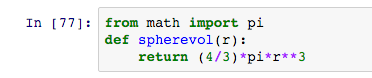
\includegraphics[width=.55\textwidth]{spherevol.png}

\end{document}